\capitulo{4}{Metodología}

\setsecnumdepth{subsubsection}

\section{Descripción de los datos}
En este apartado se detalla la información obtenida de las tres bases de datos públicas de referencia utilizadas en este proyecto: DrugBank \cite{drugbank}, SIDER \cite{sider} y CIMA \cite{cima}.

Además se especifican los criterios de selección y filtrado de datos para la realización de los conjuntos de datos creados.
\paragraph{SIDER}
Se descargaron los registros estructurados en formato TSV correspondientes a efectos adversos (\texttt{meddra\_all\_se.tsv}), frecuencias de aparición (\texttt{meddra\_freq.tsv}) y mapeo de nombres (\texttt{drug\_names.tsv}). A través de un cruce indexado por identificador de compuesto (flat), se unificó la información para calcular la frecuencia media de aparición de cada síntoma recogido en el documento llamado \texttt{efectos\_adversos.csv}.
Mas tarde se incluye a el documento mencionado una columna adiccional con los códigos ATC únicos de cada principio activo obtenidos del documento llamado \texttt{drug\_atc.tsv} para poder facilitar la interoperabilidad con las siguientes bases de datos consultadas y el fácil acceso por parte de la herramienta generada.

\paragraph{DrugBank}
Se utilizó como la ontología central para el modelado de fármacos, dianas y rutas metabólicas. La adquisición se realizó mediante la descarga de su base de datos completa en formato XML (\texttt{full\_database.xml}), procesando mediante parsing un total de 10.162 principios activos únicos. De este repositorio se extrajeron de forma dirigida los campos de identificador binario (\texttt{drugbank\_id}), nombre genérico, sinónimos comerciales, tipos de interacción (diana o enzima), nombre del gen codificante y acciones farmacodinámicas asociadas.

\paragraph{CIMA}
Se extrajo e iteró la base de datos estructurada de prescripción (Prescripcion.xml) junto a sus diccionarios auxiliares de formas farmacéuticas y situaciones de registro. Esto permitió trabajar con 30.232 registros de medicamentos autorizados en España. De las cuales, como se explica mas adelante se intentarán obtener las fichas técnicas de 665 registros concretos.

\subsection{Criterio inclusión/exclusión}
Para acotar el alcance del proyecto se aplicaron de forma secuencial los siguientes criterios de selección (filtros de inclusión/exclusión):
\begin{itemize}
    \item \textbf{Restricción del Perfil Enzimático (Top 6 CYP).} Tras analizar la distribución de frecuencias de las enzimas en DrugBank, se constató que la familia del citocromo P450 concentraba la inmensa mayoría de las rutas metabólicas de fase I. Se acotó el diseño computacional a las seis isoenzimas con mayor impacto y frecuencia de aparición (visible en la tabla \ref{fig:frecuencia_cyp} creada en un notebook auxiliar no incluido): CYP3A4, CYP2C9, CYP2D6, CYP1A2, CYP2C19 y CYP3A5. Se incluyó CYP3A5 debido a su estrecha relación con CYP3A4. 
    \item \textbf{Criterio Base de Datos de CIMA.} De estos registros inicialmente extraídos se excluyeron los medicamentos compuestos por mas de un principio activo. Esto permitió aislar 25.453 medicamentos monofármaco. De estos, eliminando duplicidades de presentaciones comerciales, se identificaron 2.100 principios activos puros validados para el mercado español.
    \item \textbf{Filtrado Ontológico de Efectos Adversos.} Por último para el procesamiento de SIDER, se aplicó un criterio de exclusión sobre la columna \texttt{meddra\_type}, descartando los términos generales (LLT) y limitando la Ingesta únicamente a los Términos Preferidos (PT, Preferred Terms). Esto redujo el conjunto final a 968 compuestos químicos con perfiles de toxicidad normalizados y frecuencias cuantitativas verificadas.
\end{itemize}

\begin{figure}[h]
    \centering
    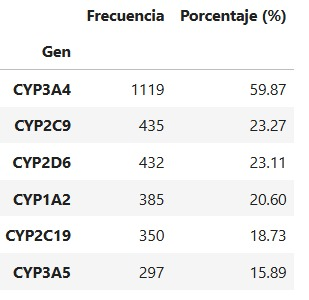
\includegraphics[width=0.35\textwidth]{img/frecuencias_cyp.jpeg} 
    \caption{Resumen frecuencia de aparición de las enzimas seleccionadas en DrugBank}
    \label{fig:frecuencia_cyp}
\end{figure}

\subsection{Criterio de resolución de ambiguedades}
Cuando un principio activo presentaba múltiples enzimas del citocromo P450 seleccionadas en DrugBank de forma simultánea, el sistema informático se encontraba ante una ambigüedad matemática para determinar el riesgo de interacción asociado. Por tanto, se intentará detectar la via metabólica principal que sigue cada uno de los 753 principios activos en los que esto sucede.

Para ello se filtran tan solo los que tienen como acción sustrato \footnote{sustrato: que posean como acción sustrato significa que la enzima actúa de manera directa sobre una molécula específica para transformarla químicamente \cite{biolan_health_enzimas}}, lo que reduce el conjunto a 665 registros, después, se seleccionaron de forma programática los códigos ATC coincidentes entre DrugBank y CIMA de esos principios activos, lo que nos reduce un más el conjunto de datos a 418 registros. Sobre estos se ejecutó un algoritmo de extracción (mediante web scraping \footnote{Web scrapping: técnica que se utilizada para extraer información de sitios web de manera automatizada \cite{esic_web_scraping}.}) sobre sus respectivas fichas técnicas oficiales. En el presente proyecto primero se descargaron de manera programática cada uno de los pdfs correspondientes a las fichas técnicas (en caso de encontrarse) de cada principio activo problema (en un periodo prolongado de tiempo, evitando de esta manera errores del tipo 429 \footnote{error 429: too many requests, significa que el servidor rechaza temporalmente la conexión por saturación de tráfico (muchas solicitudes en poco tiempo).}). 

Esta información textual extraída fue procesada mediante modelos de lenguaje vectorizados (NotebookLM y ChatGPT) para determinar cuál de las enzimas registradas ejercía el rol de vía metabólica principal (categorizada como prioridad = 1) frente a las secundarias y su posterior creación de un dataframe con esta información con el objetivo de poder incluirlo con los datos extraídos de DrugBank. Cuando no fue posible encontrar ninguna via principal se categorizan a todas las presentes en ese principio activo como prioridad = 0.

Debido a las limitaciones temporales y al elevado volumen de documentación bibliográfica por analizar, se optó por el uso de herramientas de Inteligencia Artificial (IA) para la identificación de la enzima principal. En concreto, se seleccionó NotebookLM para la revisión de las fichas técnicas, dado que este modelo opera exclusivamente con las fuentes de información suministradas por el usuario (con un límite de 50 documentos por consulta), lo que minimiza el riesgo de alucinaciones.

El procedimiento consistió en la introducción secuencial de bloques de registros previamente segmentados. A partir de estos datos, se consultó al modelo sobre la presencia de la enzima principal para cada fármaco; en caso de ausencia de resultados, se parametrizó la respuesta para devolver el valor None. Finalmente, con el objetivo de optimizar el procesamiento de datos y evitar la transcripción manual, se empleó ChatGPT para la estructuración y conversión de los resultados obtenidos en un dataframe(df) \footnote{dataframe (df): estructura de datos que los organiza en una tabla bidimensional de filas y columnas, similar a un excel}. 

Posteriormente, se filtró el dataframe mediante la exclusión de aquellos fármacos cuya enzima principal no coincidía con las seleccionadas para el presente proyecto. Asimismo, en los casos donde se identificaron simultáneamente las enzimas CYP3A4 y CYP3A5 como principales, se optó por descartar esta última. Dicha decisión se fundamenta en que, debido a la alta prevalencia de polimorfismos genéticos asociados a CYP3A5, la mayoría de la población humana no expresa de forma funcional esta isoenzima.

\section{Técnicas y herramientas.}
Para el desarrollo del sistema de detección e interpretación de interacciones farmacológicas, se ha diseñado un flujo de trabajo enfocado en la ingeniería de datos biomédicos, el procesamiento de lenguaje natural y la visualización analítica. A continuación, se detallan las técnicas e infraestructuras de software implementadas:

\subsection{Entorno de Programación y Librerías Científicas}
La extracción y procesamiento de los datos y la lógica computacional, se han implemantado bajo el lenguaje de programación Python. Para la manipulación y estructuración matricial de la información se ha utilizado la librería de código abierto Pandas, permitiendo realizar operaciones complejas de unificación (merge), filtrado por condiciones y agregación de variables bioinformáticas. Asimismo, se ha empleado la biblioteca nativa ElementTree (ET) para la lectura y extracción eficiente en términos de memoria de archivos extensos estructurados en formato XML.

\subsection{Técnicas de Extracción y Consolidación de Datos}
Debido a la heterogeneidad y procedencia de las fuentes originales, ha sido necesario aplicar diferentes técnicas de ingeniería de datos para unificar los identificadores de los principios activos y posibilitar la interoperabilidad entre las diferentes fuentes:

\begin{itemize}
    \item \textbf{Estandarización de Identificadores mediante Código ATC.} Para resolver las discrepancias nomenclátricas entre las bases de datos americanas, europeas y nacionales, se ha utilizado el sistema de clasificación jerárquica de la Organización Mundial de la Salud (OMS). Los códigos ATC se han empleado como clave primaria universal para cruzar e integrar registros procedentes de plataformas inicialmente inconexas.
    \item \textbf{Procesamiento de Estructuras Jerárquicas Complejas.} Dado que un único fármaco puede presentar múltiples acciones biológicas o códigos de indexación anatómica, se ha utilizado la técnica de explosión de colecciones en filas (exploding) sobre vectores previamente divididos. Esto ha permitido aislar cada tupla "principio activo - acción"  o "principio activo - código ATC"  de manera simplificada para evitar sesgos en el análisis posterior.
    \item \textbf{Técnicas de Web Scraping y Peticiones Programáticas Controladas.} La recopilación de las fichas técnicas oficiales de CIMA se ha realizado de forma automatizada mediante la biblioteca Requests. Para evitar sobrecargar los servidores gubernamentales de la AEMPS y prevenir la aparición de errores del tipo 429, por tanto, la columna llamada 'Prioridad' en el documento \texttt{DDI\_sea.csv} se ha implementado de forma asíncrona segmentando el volumen total (418) en bloques reducidos de 40 registros e introduciendo retrasos controlados en la ejecución.
\end{itemize}



\section{Metodología de Ingeniería del Software}
En esta sección se detalla el marco metodológico, el conjunto de tecnologías y el flujo de arquitectura de software implementados para el desarrollo, despliegue y puesta en producción de la interfaz interactiva del presente proyecto.

\subsection*{Framework de visualización: Dash}
Para la construcción de la interfaz interactiva y la representación de los datos analizados, se seleccionó el entorno de desarrollo \textit{Plotly Dash}. Dash es un framework de código abierto basado en Python, lo que simplifica significativamente su programación al omitir la necesidad de requerir conocimientos avanzados en desarrollo \textit{frontend} \footnote{Desarrollo frontend: subárea de la ingeniería de software enfocada en el diseño, estructura y creación de la interfaz visual de un sitio web o aplicación con la que interactúa el usuario.}.

La elección de esta herramienta frente a otras alternativas se fundamentó en su capacidad para diseñar soluciones ágiles. A diferencia de las plataformas comerciales o herramientas ya existentes para la consulta de interacciones farmacológicas (las cuales suelen integrar volúmenes masivos de información que pueden saturar la toma de decisiones del facultativo), uno de los objetivos de este proyecto requería una arquitectura visualmente eficiente. De este modo, Dash permitió estructurar un cuadro de mando donde, el profesional sanitario puede identificar los datos críticos esenciales, incluyendo la información ampliada bajo demanda y las alternativas farmacológicas consideradas seguras.

\subsection*{Renderización de la visualización: Render}
Una vez completado el desarrollo local de la interfaz interactiva, se procedió a su despliegue en un entorno de producción a través de la plataforma Render \cite{render}. La selección de esta infraestructura frente a otras alternativas se justificó por su alto grado de automatización y su capacidad de integración continua con repositorios de control de versiones. Esto permitió agilizar los tiempos de computación, garantizando la disponibilidad inmediata y estable de la aplicación web de cara a la fase de evaluación y defensa ante el tribunal examinador.



